\subsection{Transaction Anonymity}
\label{trans}
Communication anonymity is necessary but not sufficient for
anonymous trading, as the cryptographic objectives of authentication and legitimacy are not fulfilled. We suggest using cryptographic techniques from distributed ledgers, \textit{blockchains} and cryptocurrencies. The most adopted of which is the Bitcoin blockchain and currency. It allows for very simple digital cash spending but has serious privacy and anonymity flaws~\cite{Barber2012,Reid2013,apostolaki2017}. Additionally, Biryukov and Pustogarov, 2015, show that using Bitcoin over the Tor network opens an entirely new attack surface~\cite{biryukov2015}. Solutions to the tracing and identification problems identified by these researchers have been proposed and implemented in alternative cryptocurrency protocols: mixing using ring signatures and zero-knowledge proofs~\cite{miers2013zerocoin,cryptonote}. 

\subsubsection{Mixing Through Ring Signatures}
The CryptoNote protocol prevents tracing assets back to their original owners by
mixing together multiple incoming transactions and multiple outgoing
transactions. This service thus hides the connections between the
prosumers and the anonymous addresses. Mixing requires the possibility to create new wallets at will, something that is generally recommended upon any cryptocurrency transfer and it requires the existence of a sufficient number of participants in the network. These protocols enable participants to
mix assets with each other, thereby eliminating the need for a trusted
third party. Monero is an example of a cryptocurrency that provides built-in mixing services by implementing the CryptoNote protocol~\cite{cryptoeprint:2015:1098}. There are however alternative implementations of mixing protocols such as CoinShuffle~\cite{ruffing2014coinshuffle} or
Xim~\cite{bissias2014sybil}.

The CryptoNote protocol achieves two objectives:  
\begin{compactenum}
\item Untraceable transactions - \textit{for each incoming transaction all possible senders are equiprobable}. 
\item Unlinkable transactions - \textit{for any two outgoing transactions it is impossible to prove they were
sent to the same person}~\cite{cryptonote}.
\end{compactenum}

Group signatures were first introduced by Chaum and van Heyst, 1991,~\cite{Chaum1991} and then built upon by Rivest \textit{et al.}, 2001~\cite{Rivest2001}. The basis for anonymity in the CryptoNote protocol, however, is a slightly modified version of the \textit{Traceable ring signature} algorithm by Fukisaki and Suzuki, 2007~\cite{Fujisaki2007}. The algorithm allows a member of a group to send a transaction in such a way that it is impossible for a receiver to know any more about the sender than that it came from a group member without the use of a central authority.

Unlinkability is achieved by \textit{one-time ring signatures}, making use of four algorithms: \textbf{GEN, SIG, VER, LNK}. The general principle of the unconditional unlinkability is that a sender signs a transaction using a public key and a key image generated by \textbf{GEN} and produces a one-time ring signature using \textbf{SIG} and the public key pair and key image. \textbf{SIG} makes use of a non-interactive zero-knowledge proof which the verifier(s) then use to check the signature in \textbf{VER}. If the signature is valid, the verifier checks if the key image has been used in previous transactions, which mean that the same secret key was used to produce multiple signatures. She does that by running the algorithm \textbf{LNK}. Assuming that the mapping of the secret key to the key image is a one-way injection, it is certain that: \textbf{A.} The signer is not identifiable by way of recovering the secret key from the key image. \textbf{B.} The signer cannot create another key image with the same secret key. 

Additionally, if the receiver and sender have randomly generated, unique and new addresses, the Diffie-Hellman protocol can be used to generate a new pair of public-private keys. This is how untraceability of public keys is achieved. The sender should generate ephemeral keys for each transfer, enabling only the receiver to recover the corresponding private key. As an illustrative example, in Figure \ref{fig:ringsigs}, a schematic diagram shows households A, B and C signing a transaction since they are part of the same ring. A ring would, in reality, be many more households, not necessarily of the same microgrid. Let's assume that A is the true origin of the transaction. When E receives the transaction, the only thing that E can know with certainty is that one of A, B or C initiated the transaction. To increase the transaction anonymity further, a second, third or n rounds of ring signatures can be algorithmically imposed upon the network. With each round of signing parties, the group of potential origins grows linearly. Notably, the ring signature algorithm by Fujisaki and Suzuki, \cite{Fujisaki2007}, has been published in a peer-reviewed paper. This can be compared favorably to many cryptocurrency protocols which are simply published as white papers without any formal review-process~\cite{cryptonote}.
In practice, a transaction using the mixing service should be performed in the following way to ensure anonymity:


It is also possible for household A that it paid prosumer B for energy by either disclosing the random number used in the generation of the one-time public destination key used in that transaction to B. Or she can use any other kind of zero-knowledge protocol to prove she knows the random number. The ring signatures would also allow the auditing of transactions by, for example, the DSO. This would be achieved by prosumer B giving the tracking key or truncated address to the DSO, who would then be able to link all incoming transactions to B.

\subsubsection{Mixing through Zero-Knowledge Proofs}
Zero-knowledge proofs (ZKP) are ways for a person to prove the knowledge of some specific fact to a verifier, without actually having to disclose the knowledge. Blum \textit{et al.} provided non-interactive ZKPs (NIZK) in 1988 \cite{Blum:1988:NZA:62212.62222}, where the prover and verifier don't have to interact or communicate directly with each other. The Zerocoin protocol \cite{miers2013zerocoin} outlines a way how NIZKs can achieve the untraceability objective of the previous section and it ensures that no double-spending is allowed.\footnote{Each coin in the protocol is identified uniquely by a serial number.} Zerocoin is a protocol for the decentralized mixing of coins, so that they can not be traced, or \textit{tainted}. However, senders and destinations can still be identified~\cite{miers2013zerocoin}.  Luckily, Zerocash~\cite{Sasson:2014:ZDA:2650286.2650810} extends the NIZK functionality to allow for anonymous transactions, anonymous balances and coins, improved performance of transactions and sending of assets to a receivers fixed address without action required from the receiver. Zerocash makes use of a more efficient version of the NIZK, used in Zerocoin, called ZK \textit{Succinct Non-interactive ARguments of Knowledge} (zk-SNARK). 
% It features the algorithms: \textbf{Setup($1^\lambda$)}$\rightarrow \textit{params}$, \textbf{Mint(}\textit{params})$\rightarrow \textit{(c,skc)}$, \textbf{Spend}(\textit{params, c, skc, R, \textbf{C}})$\rightarrow(\pi, S)$ and \textbf{Verify}(\textit{params, $\pi$, S, R, \textbf{C}})$\rightarrow$$\{$0,1$\}$. The \textbf{Setup} function takes a secret parameter and returns a global public set of parameters and description of the set of coins. It is only executed once in the lifetime of the scheme, and the authors of the protocol recommend the usage of a trusted party for this. \textbf{Mint} is used to create coins from the coin set, given the parameters. \textbf{Spend} and \textbf{Verify} are executed by a sender and a receiver, respectively at the beginning and end of each transaction.

The Zerocash-scheme could be carried out using a simple messaging board, but would not be safe in practice since information might be manipulated or the owner of said board might collude etc. Therefore, an immutable, decentralized data storage, governed by the consensus of its peers is required to assure the secure transmission of information. The blockchain provides such a structure. 
% \begin{enumerate}[noitemsep,topsep=-\parskip]
% \item A mints a new message by generating a new random serial number $S$ of value $V$ and commits to it.
% \item The commitment, $C$, is such that only the secret message $m$ can reveal $S$.
% \item A then mints a second message by generating a new serial number $S_m$ so that the commitment $C$ is decrypted by the message $m$. 
% \item A posts the commitments to a blockchain along with the corresponding value in cryptocurrency.
% \item B has sold energy during the last timeperiod with references ($m_i,\dots m_j$) and has thereby $j-i$ number of references to scan the blockchain for.
% \item To redeem the payment, B produces a ZKP $\pi$ for the following statements:
% \begin{enumerate}[noitemsep,topsep=-\parskip]
% \item B knows a tuple ($C$) from all valid commitments available and
% \item B knows the secret $m$ such that the commitment ($C$) opens to ($S$) 
% \end{enumerate}
% \item B can now post a 'spend'-transaction containing ($S,\pi$) on the blockchain.
% \item The other users verify $\pi$ and ensure that ($S$) didn't occur already in the history of transactions.
% \item If correct, then the blockchain protocol allows B to collect cryptocurrency of value $V$. 
% \end{enumerate}
% This requires B to know all references to energy transactions that are outstanding (and coming from prosumer B) to date, and to be able to compare them to the available, valid commitments. 

\subsubsection{Threats and weaknesses in Ring Signature- and Zero-Knowledge Proof-schemes}
\label{transthreat} 
\begin{figure}[t]
\centering
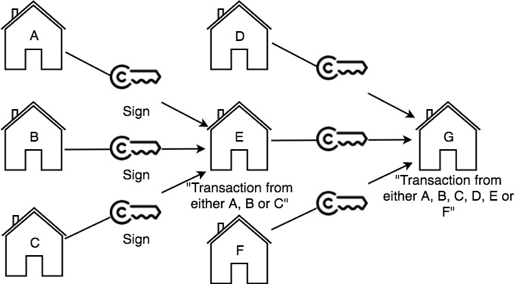
\includegraphics[width=\columnwidth]{ringsigs.png}
\caption{Visualization of untraceability in ring signatures in smart meter-based energy trading and the potential deductions of origin of the transaction by a single household in the chain of signatures.}\label{fig:ringsigs}
\end{figure}
When applying either ring signatures or zero-knowledge SNARKs to PETra, potential weaknesses or attacks need to be considered.A potential threat to ring signatures is when a large amount of the unspent transactions are owned by an adversary or when insufficient amounts of signatures are included in a ring. When a prosumer A wishes to select a group of signatures to sign her transaction as well, then it is likely that she will select many of the transactions from the adversary. Assuming the adversary spends his outputs without \textit{mixing}\footnote{The number of other signatures used in the ring.}, then A's transaction is exposed as well~\cite{monero2014}. Recent research  also show that up to 65\% of Monero transactions are trivially traceable using one attack. They also exposes two more attacks that have been amended in the latest versions of the protocol, lowering the amount of transactions traceable to 20\%~\cite{monero2014,DBLP:journals/corr/MillerMLN17}.

One of the main weaknesses of the Zerocash-based protocol is that for each private transaction, a costly zk-SNARK needs to be computed. But that is not a threat to anonymity, just a practical reason why it might be difficult to run the scheme over a congested public blockchain. In \cite{Sasson:2014:ZDA:2650286.2650810}, experiments show an average time of 3 min to create the zk-SNARK for a private transaction, verifying it takes only 8.5 ms. Another large practical drawback of Zerocash is the lack of programmability and functionality that would be required in PETra. Zhang \textit{et al.} solve some of the practical flaws and amend security issues~\cite{zhangz}.

\subsubsection{Proposed Solution to Achieve Transaction Anonymity}
Applying the CryptoNote protocol to PETra could be done by performing both energy transactions and monetary transactions using ring signatures. They would be securely logged, tamper-proof and anonymous through the usage of a blockchain. Even though  some security flaws exists, as seen in the previous paragraph, the risk of identification, linking or tracing of transactions can be minimized by imposing a high minimum number of signatures per transaction. We also propose to connect the global transaction networks to augment the number of transactions and thereby limit the chance of deduction by elimination.

Applying ZKPs to PETra would require that a smart meter can encrypt and sign a transaction, transmit a proof of it to the blockchain and thus the receiver of the payment, without having to reveal the actual amount of energy or cost incurred to anyone but the receiver. This is achieved by the Zerocash-protocol and is implemented as a fork of the Bitcoin blockchain. Neither the receiver, nor any other participants can gain information about the transactions sent over the blockchain. To provide full functionality for PETra, the Zerocash-protocol would need to be implemented for the transmission of bids and asks as well as the already existing monetary transactions. The second implementation would need to be modified to transmit and link bids and asks to the payments ledger. A more straightforward but bloated structure would be to create transactions without monetary value to post a bid or an ask and then directly reference the final bid-/ask-transaction in the payment-transaction. 
% \subsubsection{Bidding Anonymity}
% Prosumers must also be able to anonymously post energy bids and asks
% on the bid storage service.  An anonymous bid (or ask) contains an ECA
% (or EPA), a price, and an anonymous communication identifier
% (\emph{e.g.}, Tor hidden service), which can be used to contact the
% bidding (or asking) prosumer.  To enforce safety requirements, the bid
% storage service must verify that the prosumer actually owns the asset
% to be traded.  To this end, the prosumer first has to prove that it
% controls the anonymous address where the asset is stored, which can be
% performed in multiple ways.

% In many distributed ledgers, an address represents a public key, and
% controlling means knowing the corresponding private key.  In this
% case, the prosumer can prove that it controls an address by signing a
% challenge, which was freshly generated by the service, with the
% private key of the address.

% \subsubsection{Smart-Meter Based Billing}
% After a prosumer has finished trading, it deposits all of its EPA,
% ECA, and FA to the smart meter by transferring them to an anonymous
% address generated by the smart meter.  Later, during timeslot $t$, the
% smart meter measures the amount of energy actually consumed (or
% produced) by the prosumer using physical sensors.  The meter can then
% compute the prosumer's bill for timeslot $t$, which will be paid to
% the DSO, as follows. \Abhishek{The safety argument should be
%   strengthened here}

% Notice that consumption assets are not used directly for billing, they are only used to enforce security and safety requirements.

